%%%%%%%%%%%%%%%%%%%%%%%%%%%%%%%%%%%%%%%%%
% Beamer Presentation
% LaTeX Template
% Version 1.0 (10/11/12)
%
% This template has been downloaded from:
% http://www.LaTeXTemplates.com
%
% License:
% CC BY-NC-SA 3.0 (http://creativecommons.org/licenses/by-nc-sa/3.0/)
%
%%%%%%%%%%%%%%%%%%%%%%%%%%%%%%%%%%%%%%%%%

%----------------------------------------------------------------------------------------
%	PACKAGES AND THEMES
%----------------------------------------------------------------------------------------

\documentclass{beamer}

\mode<presentation> {

% The Beamer class comes with a number of default slide themes
% which change the colors and layouts of slides. Below this is a list
% of all the themes, uncomment each in turn to see what they look like.



\usepackage[utf8]{inputenc}
\usepackage[T1]{fontenc}
%\usetheme{default}
%\usetheme{AnnArbor}
%\usetheme{Antibes}
%\usetheme{Bergen}
%\usetheme{Berkeley}
%\usetheme{Berlin}
%\usetheme{Boadilla}
%\usetheme{CambridgeUS}
%\usetheme{Copenhagen}
%\usetheme{Darmstadt}
%\usetheme{Dresden}
%\usetheme{Frankfurt}
%\usetheme{Goettingen}
%\usetheme{Hannover}
%\usetheme{Ilmenau}
%\usetheme{JuanLesPins}
%\usetheme{Luebeck}
\usetheme{Madrid}
%\usetheme{Malmoe}
%\usetheme{Marburg}
%\usetheme{Montpellier}
%\usetheme{PaloAlto}
%\usetheme{Pittsburgh}
%\usetheme{Rochester}
%\usetheme{Singapore}
%\usetheme{Szeged}
%\usetheme{Warsaw}

% As well as themes, the Beamer class has a number of color themes
% for any slide theme. Uncomment each of these in turn to see how it
% changes the colors of your current slide theme.

%\usecolortheme{albatross}
%\usecolortheme{beaver}
%\usecolortheme{beetle}
%\usecolortheme{crane}
%\usecolortheme{dolphin}
%\usecolortheme{dove}
%\usecolortheme{fly}
%\usecolortheme{lily}
%\usecolortheme{orchid}
%\usecolortheme{rose}
%\usecolortheme{seagull}
%\usecolortheme{seahorse}
%\usecolortheme{whale}
%\usecolortheme{wolverine}

%\setbeamertemplate{footline} % To remove the footer line in all slides uncomment this line
%\setbeamertemplate{footline}[page number] % To replace the footer line in all slides with a simple slide count uncomment this line

%\setbeamertemplate{navigation symbols}{} % To remove the navigation symbols from the bottom of all slides uncomment this line
}

\usepackage{graphicx} % Allows including images
\usepackage{booktabs} % Allows the use of \toprule, \midrule and \bottomrule in tables

%----------------------------------------------------------------------------------------
%	TITLE PAGE
%----------------------------------------------------------------------------------------

\title[Non-normative Agent Modeling]{A ontology model for investigation Non-Normative behavior in Risky Activities} 

\author{Jonathan Morris Samara,\\ Cesar Augusto Tacla} % Your name
\institute[UCLA] % Your institution as it will appear on the bottom of every slide, may be shorthand to save space
{
Universidade Tecnológica Federal do Paraná \\ % Your institution for the title page
\medskip
\textit{jonathan\_samara@hotmail.com \\ cesar.tacla@gmail.com} % Your email address
}
\date{\today} % Date, can be changed to a custom date

\begin{document}

\begin{frame}
	\titlepage
\end{frame}
\begin{frame}
	\frametitle{Context}
		  \begin{itemize}
				\item Human activity is related to following, and violation conducts norms. This generates several systemic implications for a society. An example of this involves jobs where professionals are exposed to risks to their respective lives.	  
				\item Violation of norms can have many kinds of consequences. These consequences can be slight as well can generate somebody's death. Therefore, we need models that take this behavior int consideration for the purpose of understanding certain types of relationships within the computational context. In this study we will construct a model within the formalism of ontologies.
		\end{itemize}
\end{frame}
\begin{frame}
	\frametitle{Problems}
		\begin{itemize}
			\item Within the context of multiagent systems, norms are used to define what an agent must do about certain conditions. This allows do develop a model with the purpose of representing behaviors of the human society.
			\item The representation of non-normative behaviors contributes to the creation of more realistic models. So in this study we intend do present a non-normative model for professional risk activities. With this model we intend to take int consideration how inappropriate choices can generate negative consequences in future stages of the activity.

	\end{itemize}
\end{frame}
\begin{frame}
	\frametitle{Goals}
	\begin{itemize}
		\item Identify all aspects relevant to research on a real case study of interest to the scope of this research.
		\item Investigate all existing models contributes to represent normative and non-normative behaviors.
		\item Analyze aspects of this case study that are not considered by the current models.
		\item Construct an ontology that considers aspects that where not considered in previous models.
		\item Analyze the use of the ontology to represent the case study.
	\end{itemize}
\end{frame}
\begin{frame}
	\frametitle{Solution}
	\begin{itemize}
		\item  The development of the ontology is done using \textbf{Methontology} methodology. The steps of this methodology are;
		\begin{itemize}
			\item Specify (define specifications.)
			\item Conceptualize (find patterns that can generalize several entities.)
			\item Formalize (to define the concepts whitens a formal language.)
			\item Integrate (integrate with existing models.)
			\item Implementation the ontology in some computational language and Maintenance (to correct eventual problems arises during the use of the ontology.).
		\end{itemize}
		\item UML class diagram is used to represent the ontology.
		\item The implementation of the ontology will be done using SQL relational database.
		\item We will carry out several types of query in order to evaluate if this representational model meets the needs of the case study.
	\end{itemize}
\end{frame}

\begin{frame}
	\frametitle{Results}
	
	\begin{figure}
  		\caption{Ontology to represent non-normative cases in terms of UML class diagram}
  		\centering
			  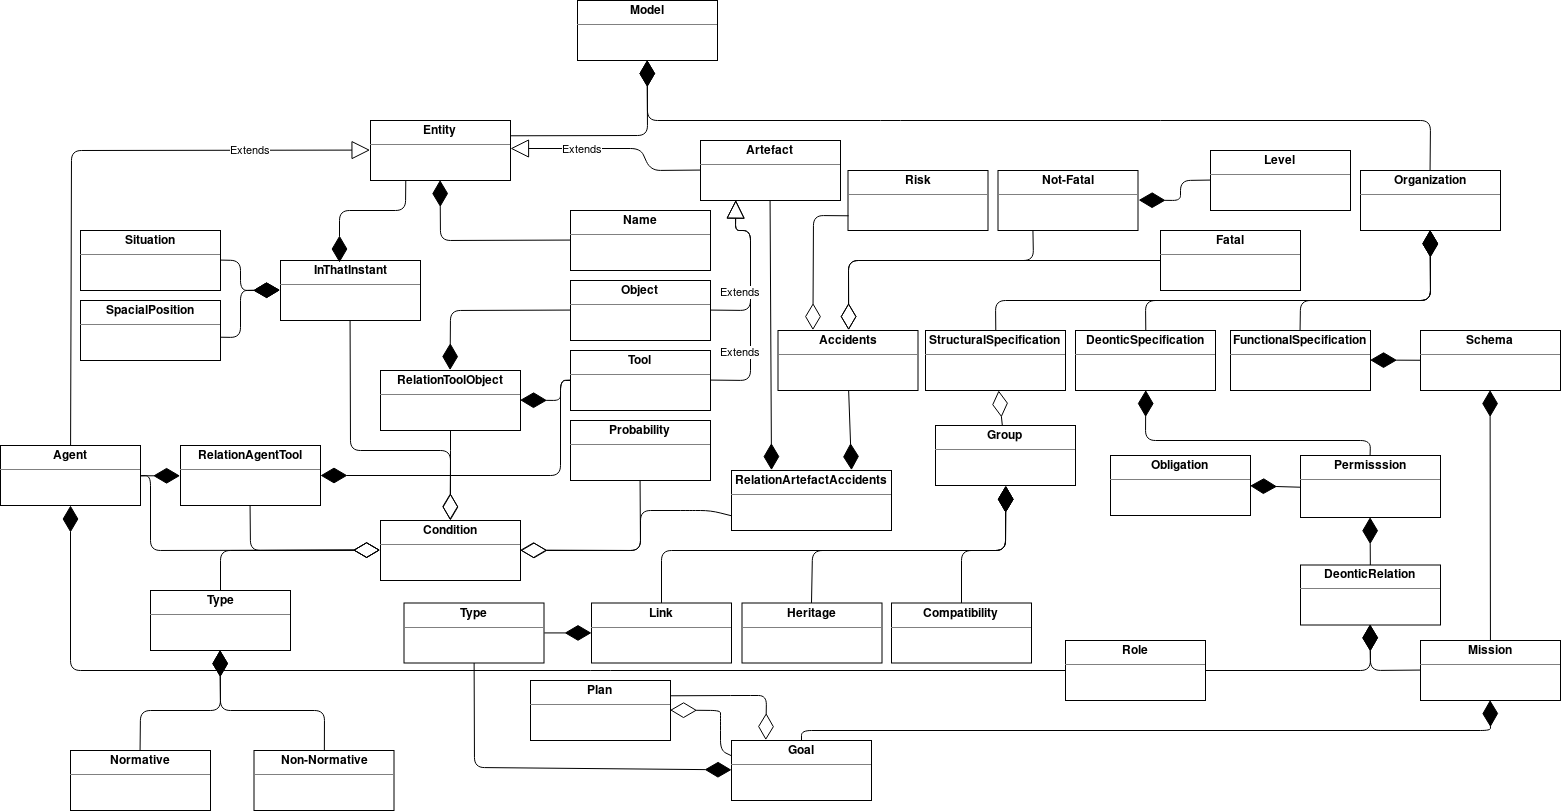
\includegraphics[width=0.8\textwidth]{uml_model_simulation}
	\end{figure}

\end{frame}
\begin{frame}
	\frametitle{Applications}
	\begin{itemize}
		\item Develop training systems for risky activities.
		\item Develop maintenance planning systems.
		\item Conduct risk analysis
		\item Analysing of direct and indirect impacts on the violation of norms with respect to the achievement of goals.
		\item Simulate maintenance practice using multiagent systems.
	\end{itemize}
\end{frame}





%----------------------------------------------------------------------------------------

\end{document} 
